\section{Results} \label{sec:results}


\subsection{Setup}
We use a local setup of spark since we are interested in I/O speed and not in distribution.
Benchmarks are performed on an Intel i7-3820QM with 12GB RAM. The disk used was a HDD.
\subsection{Scenario I}
\subsubsection{Writing Data}
In Figure \ref{fig:write-one}, we show write time for one million rows and a varying number of columns.
\begin{figure}[!htb]
\caption{Writing Time for Scenario I}
\centering
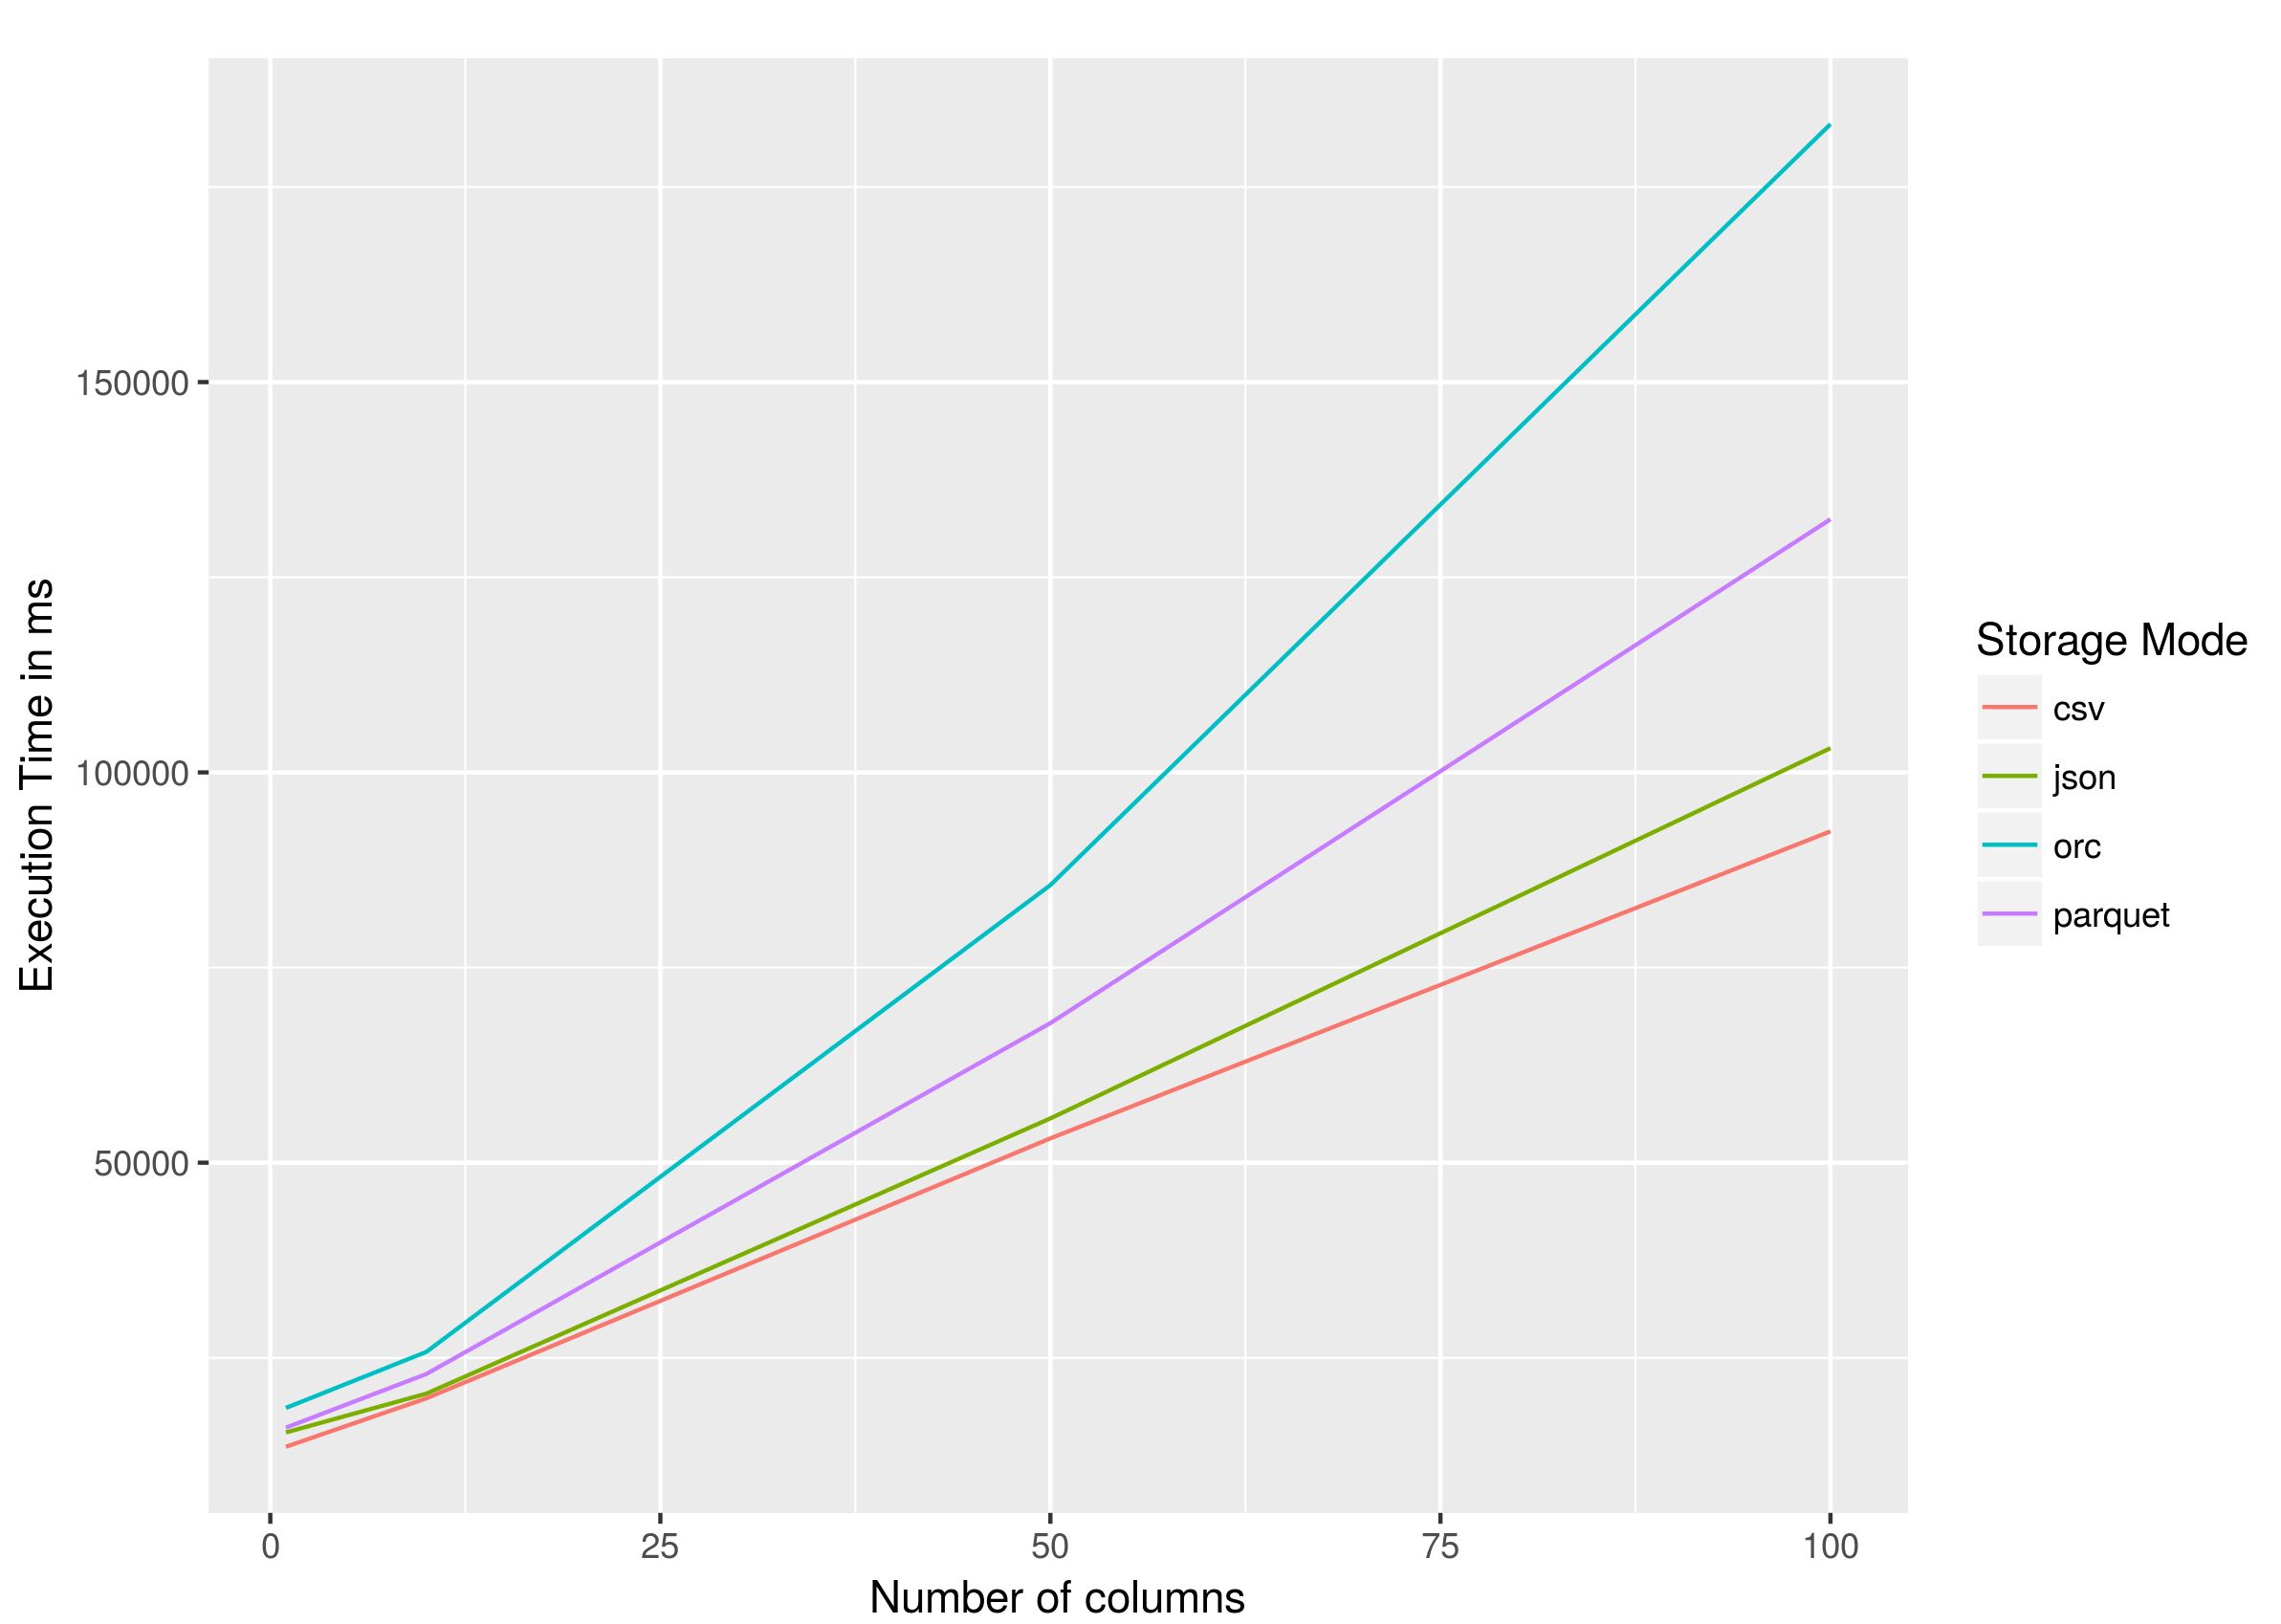
\includegraphics[width=0.75\textwidth]{write-one.png}
\label{fig:write-one}
\end{figure}

As expected, writing csv is fastest since json-files are larger. Parquet being slower is also expected.

\subsubsection{File size}
As expected, JSON uses the most hard disk space with 11 GB (for $10^6$ rows and 100 columns).
Compared with 9.5 GB for ORC, 9.8 GB for Parquet and 9.9 GB for CSV respectively, this is due to the method of schema storage in JSON.
ORC and Parquet perform better as expected since they use compression algorithms to store tables.

\subsubsection{Query}
In Figure \ref{fig:query-one}, we show the execution time of the query described in Section \ref{sec:query-one} for one million rows and a varying number of columns.

\begin{figure}[!htb]
\caption{Query Execution Time for Scenario I}
\centering
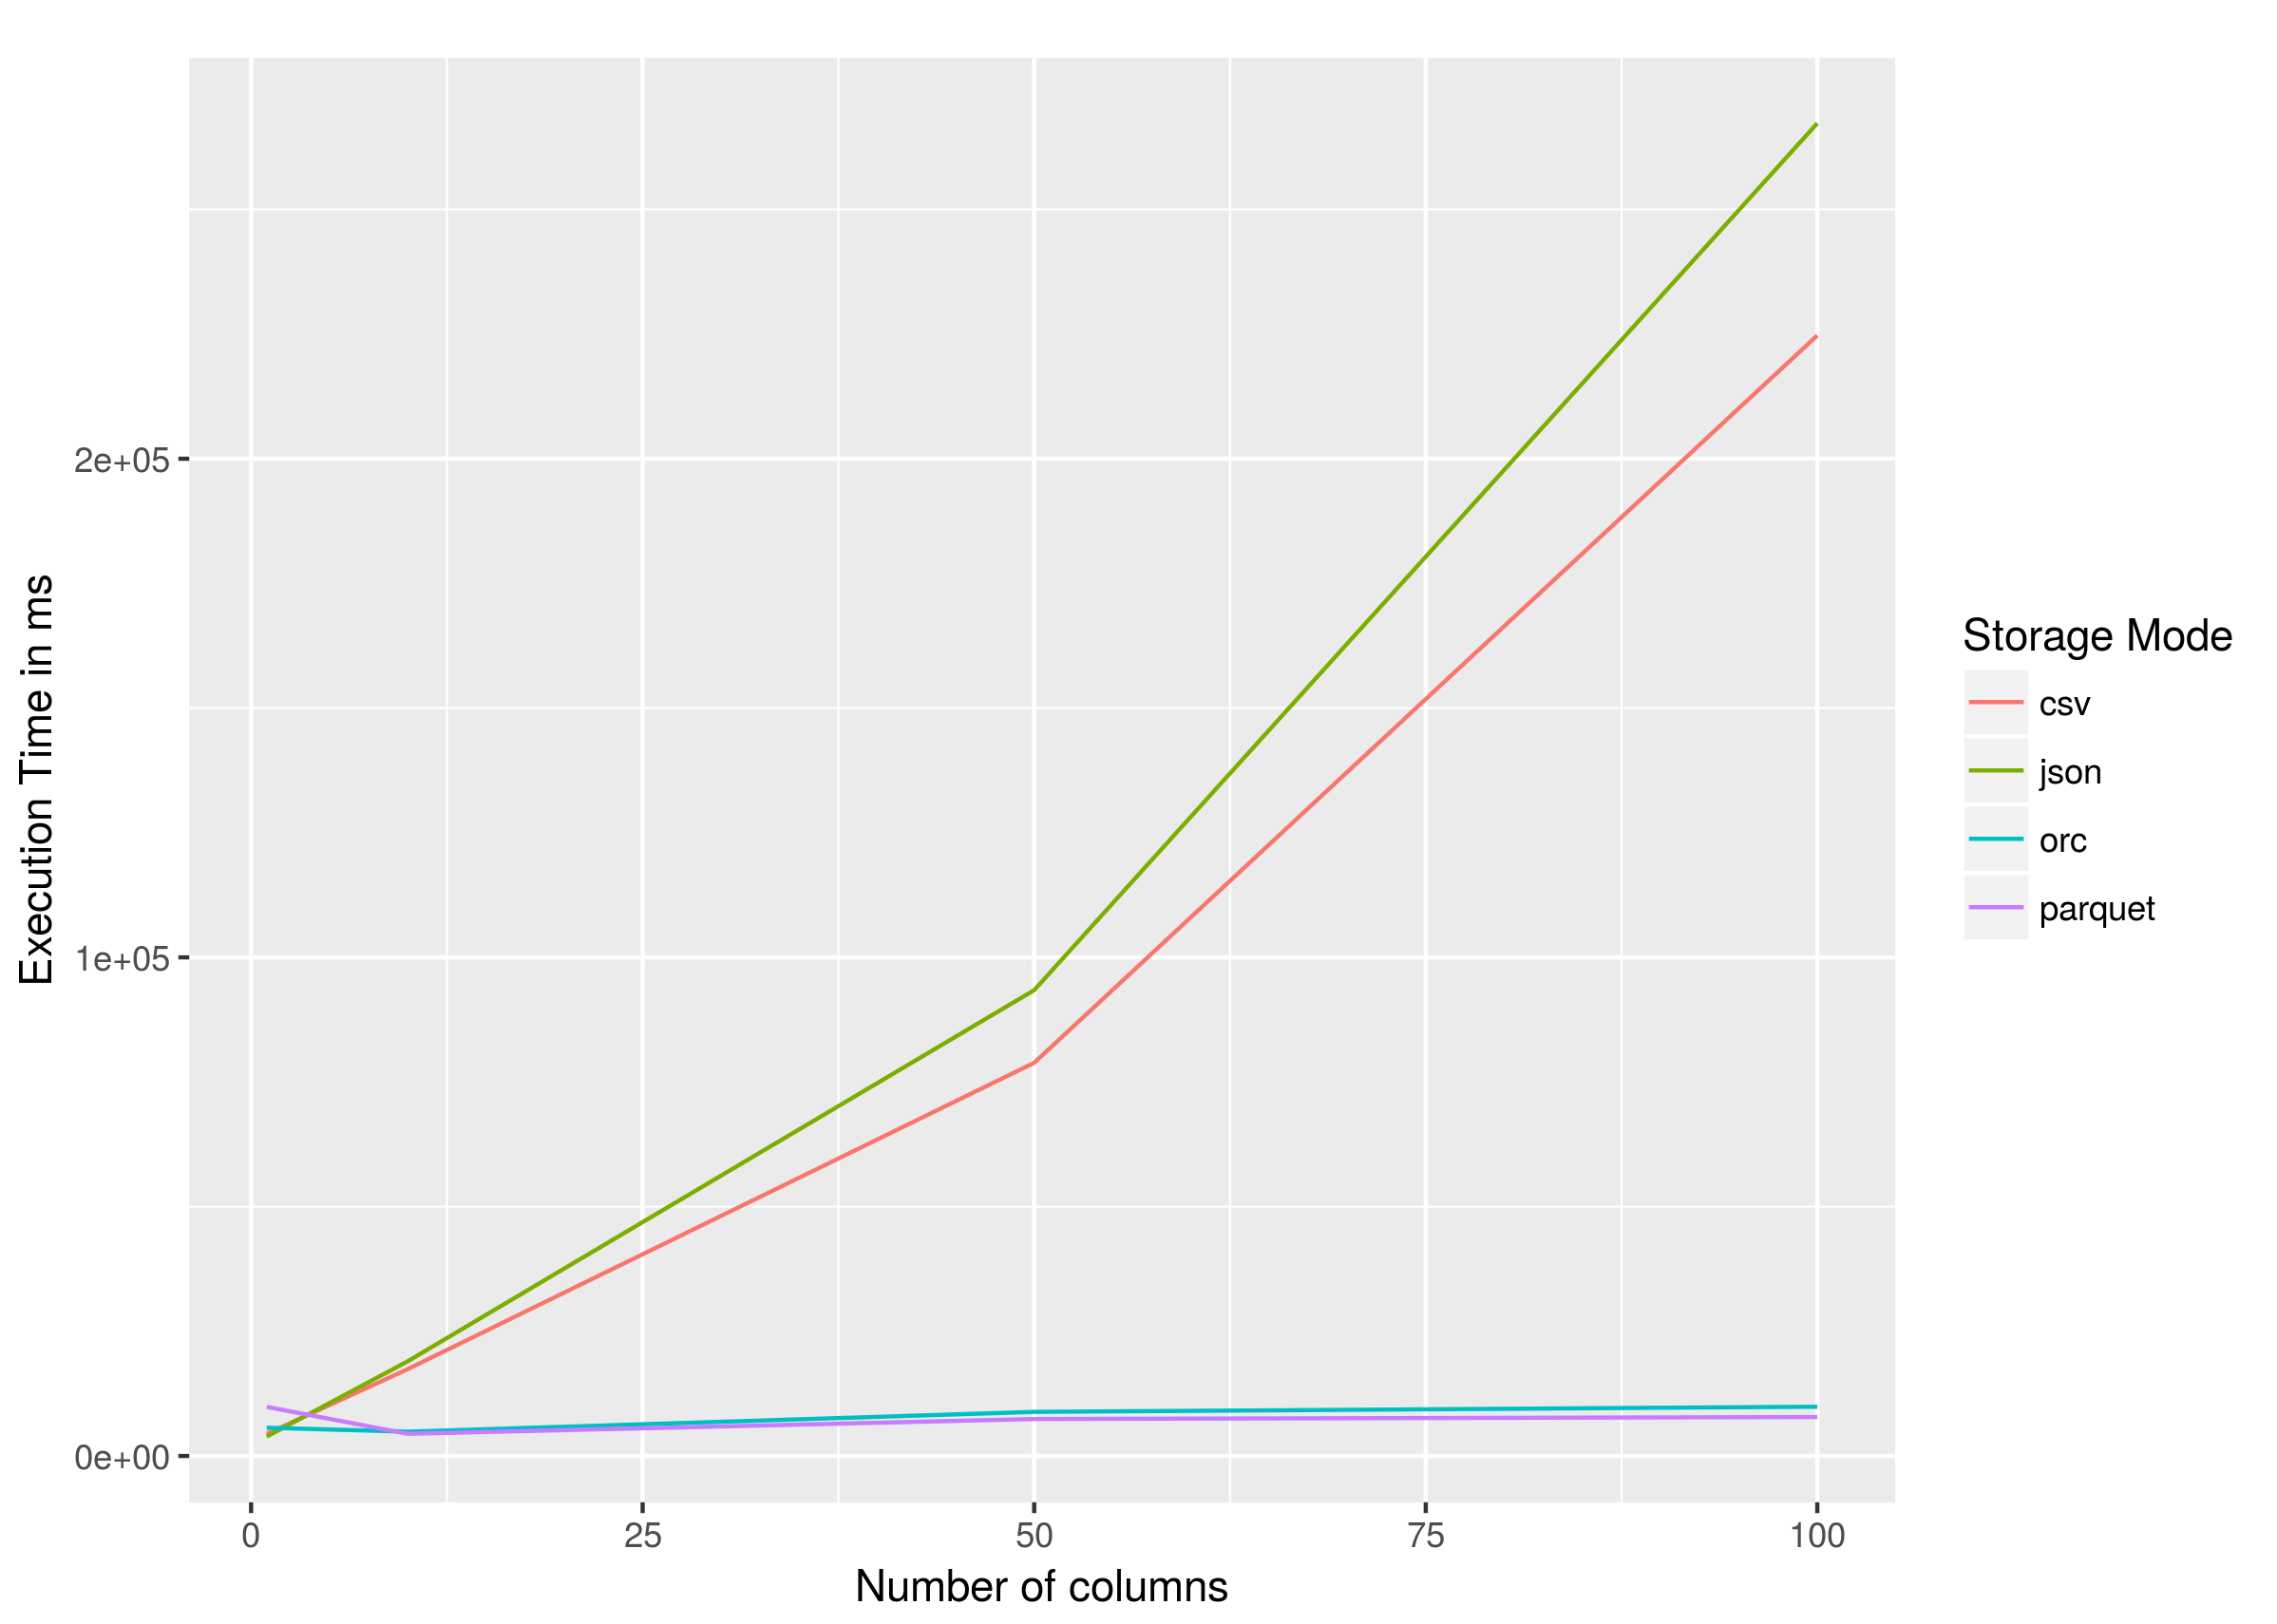
\includegraphics[width=0.75\textwidth]{query-one.png}
\label{fig:query-one}
\end{figure}

As expected, execution time for Parquet is constant as the number of column grows while execution time for JSON and CSV grows linearly.

\subsection{Scenario II}

\subsubsection{Writing Data}
In Figure \ref{fig:write-two}, we show write time for a name length of 50 and a varying number of rows.

\begin{figure}[!htb]
\caption{Writing Time for Scenario II}
\centering
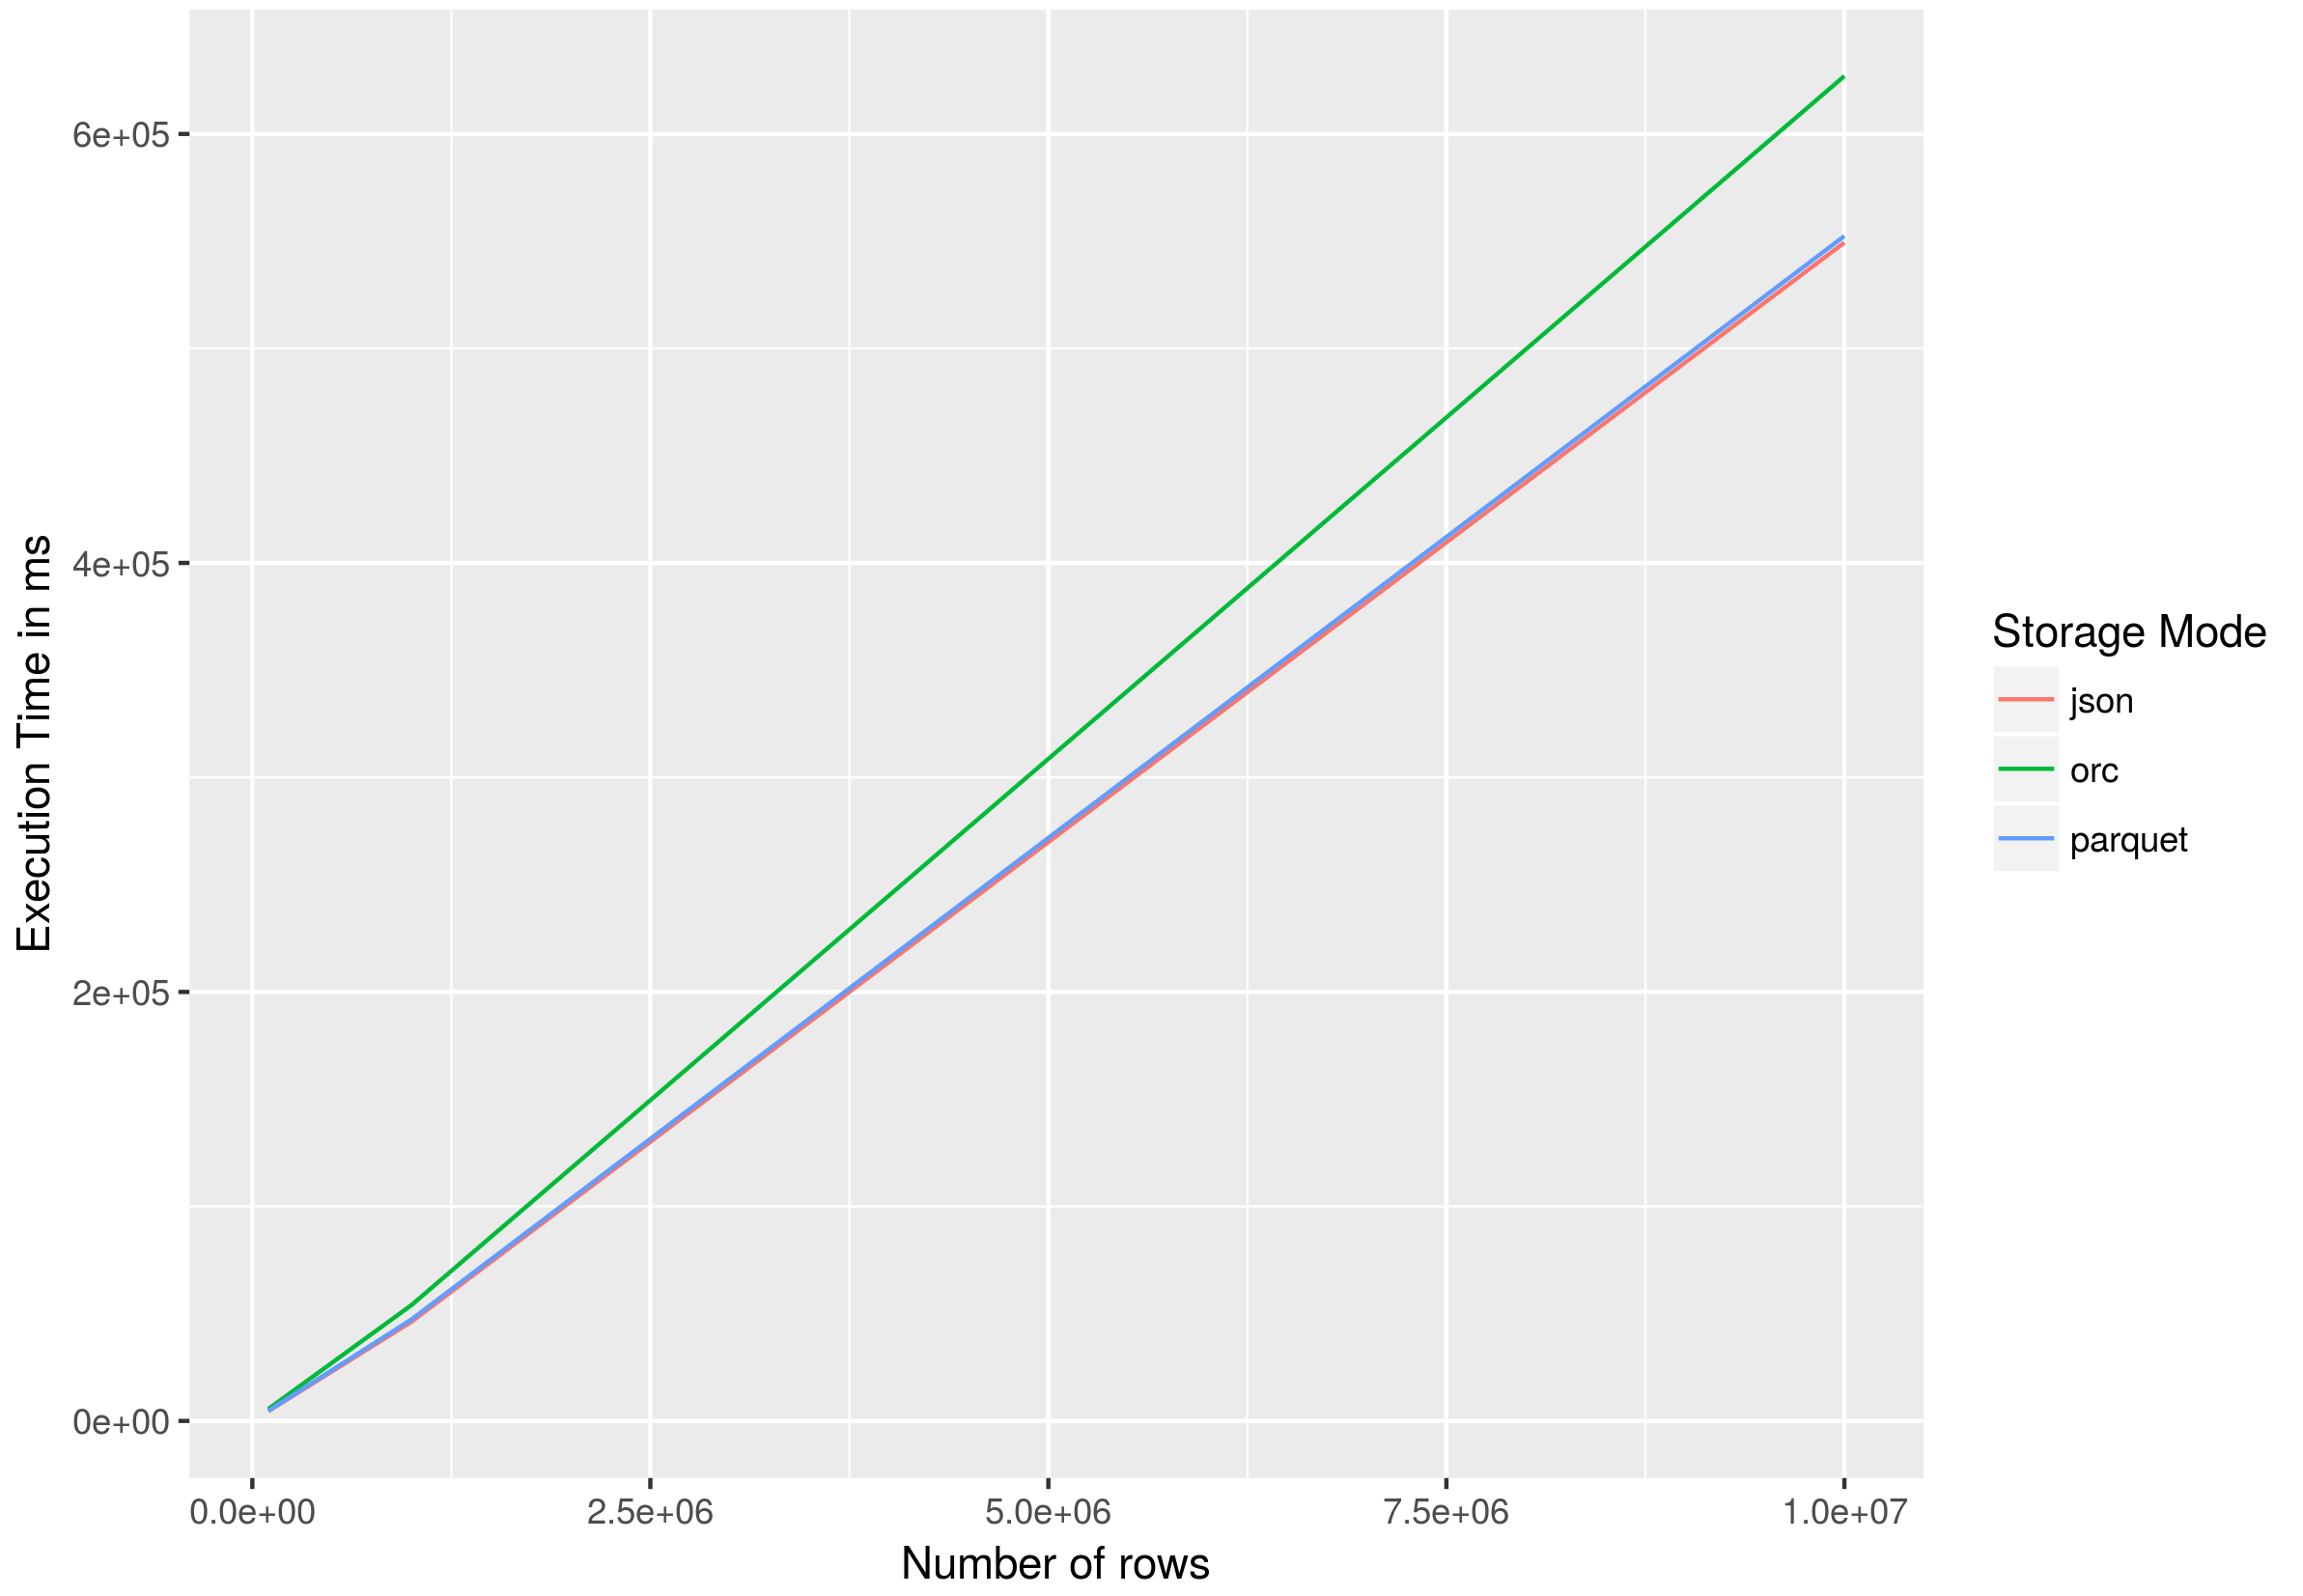
\includegraphics[width=0.75\textwidth]{write-two.png}
\label{fig:write-two}
\end{figure}

For different string lengths, the constant was that Parquet outperforms ORC and is competitive with JSON.
Again, minor write overhead is not the primary concern for most applications.

\subsubsection{File size}
As in Scenario I, JSON uses the most hard disk space with 11 GB (for $10^7$ rows and a name length of 100).
Both compression and the method of storing nested objects pays off for Parquet here as the file size is only 7.0 GB.
ORC sees similar gains and uses 6.7 GB.

\subsubsection{Query}
In Figure \ref{fig:query-two}, we show the execution time of the query described in Section \ref{sec:query-two} for a varying number of rows.

\begin{figure}[!htb]
\caption{Query Execution Time for Scenario II}
\centering
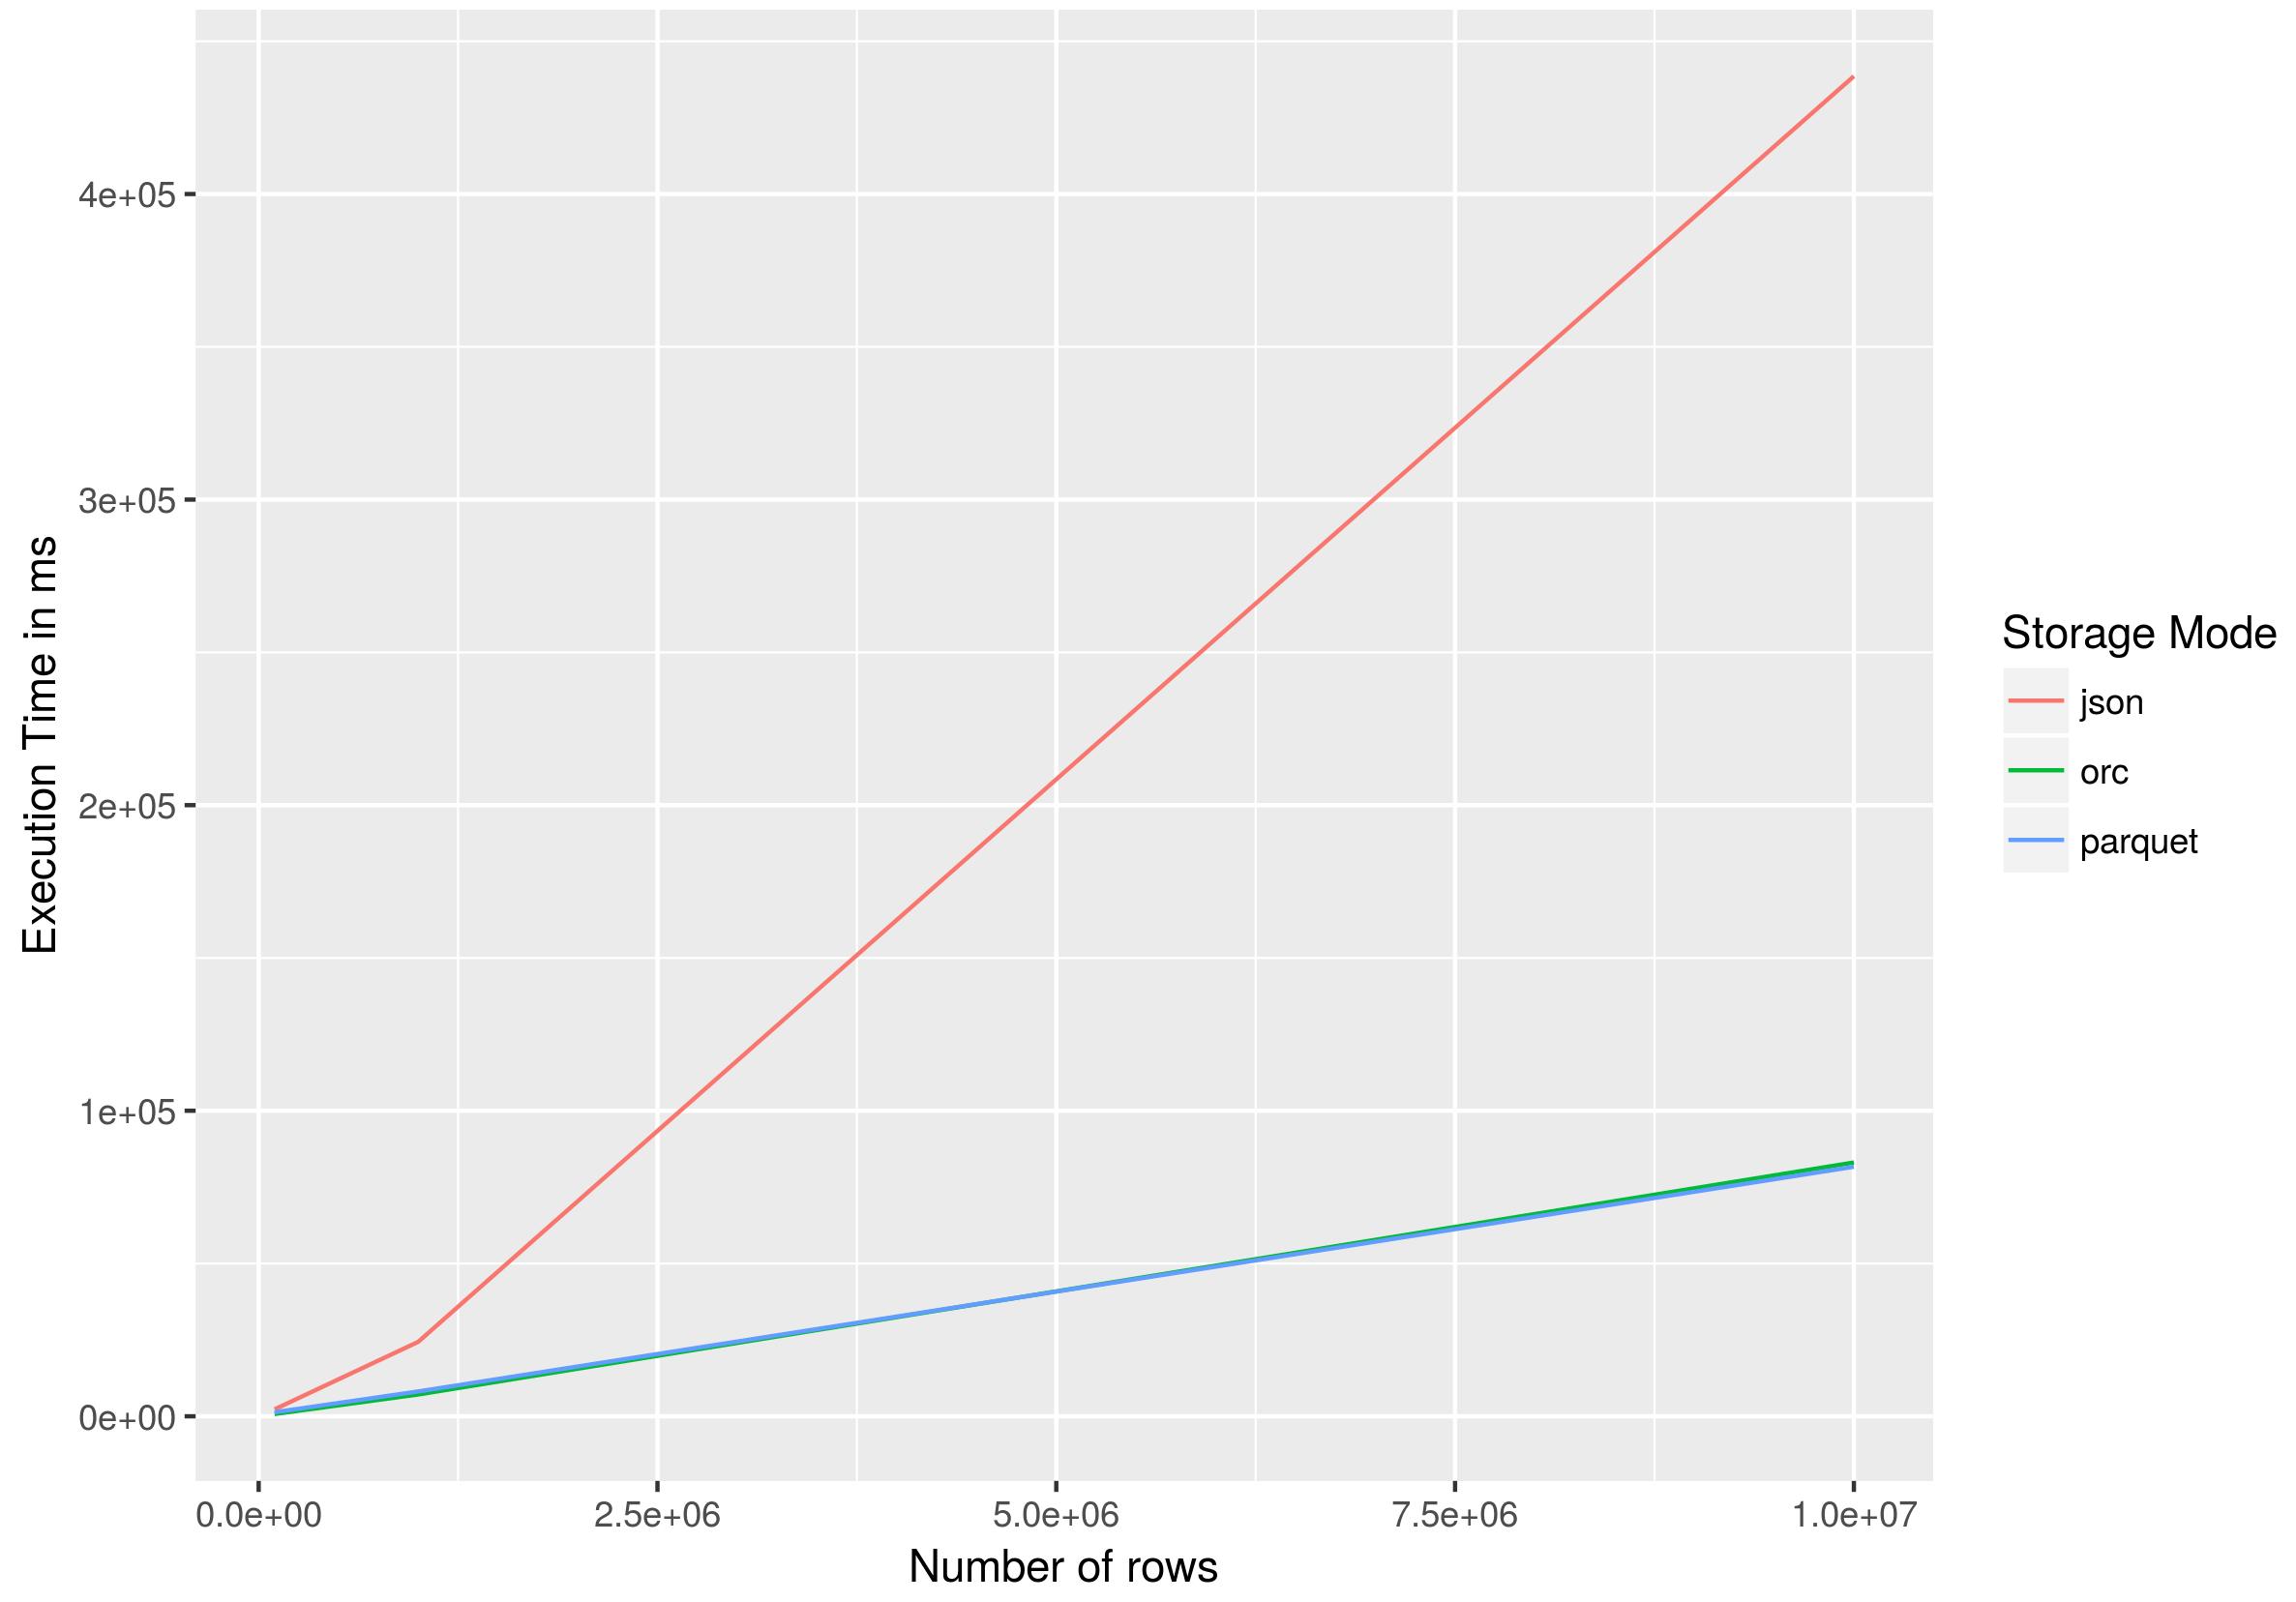
\includegraphics[width=0.75\textwidth]{query-two.png}
\label{fig:query-two}
\end{figure}

As expected, execution time for Parquet is grows linear with the number of rows but the gradient is lower.

\newpage

